\documentclass[12pt,letterpaper]{article}
\usepackage{graphicx,textcomp}
\usepackage{natbib}
\usepackage{setspace}
\usepackage{fullpage}
\usepackage{color}
\usepackage[reqno]{amsmath}
\usepackage{amsthm}
\usepackage{fancyvrb}
\usepackage{amssymb,enumerate}
\usepackage[all]{xy}
\usepackage{endnotes}
\usepackage{lscape}
\newtheorem{com}{Comment}
\usepackage{float}
\usepackage{hyperref}
\newtheorem{lem} {Lemma}
\newtheorem{prop}{Proposition}
\newtheorem{thm}{Theorem}
\newtheorem{defn}{Definition}
\newtheorem{cor}{Corollary}
\newtheorem{obs}{Observation}
\usepackage[compact]{titlesec}
\usepackage{dcolumn}
\usepackage{tikz}
\usetikzlibrary{arrows}
\usepackage{multirow}
\usepackage{xcolor}
\newcolumntype{.}{D{.}{.}{-1}}
\newcolumntype{d}[1]{D{.}{.}{#1}}
\definecolor{light-gray}{gray}{0.65}
\usepackage{url}
\usepackage{listings}
\usepackage{color}

\definecolor{codegreen}{rgb}{0,0.6,0}
\definecolor{codegray}{rgb}{0.5,0.5,0.5}
\definecolor{codepurple}{rgb}{0.58,0,0.82}
\definecolor{backcolour}{rgb}{0.95,0.95,0.92}

\lstdefinestyle{mystyle}{
	backgroundcolor=\color{backcolour},   
	commentstyle=\color{codegreen},
	keywordstyle=\color{magenta},
	numberstyle=\tiny\color{codegray},
	stringstyle=\color{codepurple},
	basicstyle=\footnotesize,
	breakatwhitespace=false,         
	breaklines=true,                 
	captionpos=b,                    
	keepspaces=true,                 
	numbers=left,                    
	numbersep=5pt,                  
	showspaces=false,                
	showstringspaces=false,
	showtabs=false,                  
	tabsize=2
}
\lstset{style=mystyle}
\newcommand{\Sref}[1]{Section~\ref{#1}}
\newtheorem{hyp}{Hypothesis}


\title{Problem Set 4 Clare Zureich}
\date{Due: November 18, 2024}
\author{Applied Stats/Quant Methods 1}


\begin{document}
	\maketitle
	\section*{Instructions}
	\begin{itemize}
		\item Please show your work! You may lose points by simply writing in the answer. If the problem requires you to execute commands in \texttt{R}, please include the code you used to get your answers. Please also include the \texttt{.R} file that contains your code. If you are not sure if work needs to be shown for a particular problem, please ask.
		\item Your homework should be submitted electronically on GitHub.
		\item This problem set is due before 23:59 on Monday November 18, 2024. No late assignments will be accepted.
	\end{itemize}



	\vspace{.5cm}
\section*{Question 1: Economics}
\vspace{.25cm}
\noindent 	
In this question, use the \texttt{prestige} dataset in the \texttt{car} library. First, run the following commands:

\begin{verbatim}
install.packages(car)
library(car)
data(Prestige)
help(Prestige)
\end{verbatim} 

	\lstinputlisting[language=R, firstline=38, lastline=41]{PS04_answers_CZ.R}

\noindent We would like to study whether individuals with higher levels of income have more prestigious jobs. Moreover, we would like to study whether professionals have more prestigious jobs than blue and white collar workers.

\newpage
\begin{enumerate}
	
	\item [(a)]
	Create a new variable \texttt{professional} by recoding the variable \texttt{type} so that professionals are coded as $1$, and blue and white collar workers are coded as $0$ (Hint: \texttt{ifelse}).
	
	\lstinputlisting[language=R, firstline=43, lastline=48]{PS04_answers_CZ.R}
	\vspace{.25cm}
	
	
	\item [(b)]
	Run a linear model with \texttt{prestige} as an outcome and \texttt{income}, \texttt{professional}, and the interaction of the two as predictors (Note: this is a continuous $\times$ dummy interaction.)
	
		\lstinputlisting[language=R, firstline=51, lastline=51]{PS04_answers_CZ.R}

	\begin{figure}[h!]\centering
	\caption{\footnotesize Income and Professional Interaction Regression.}
	\label{fig:plot_1}
	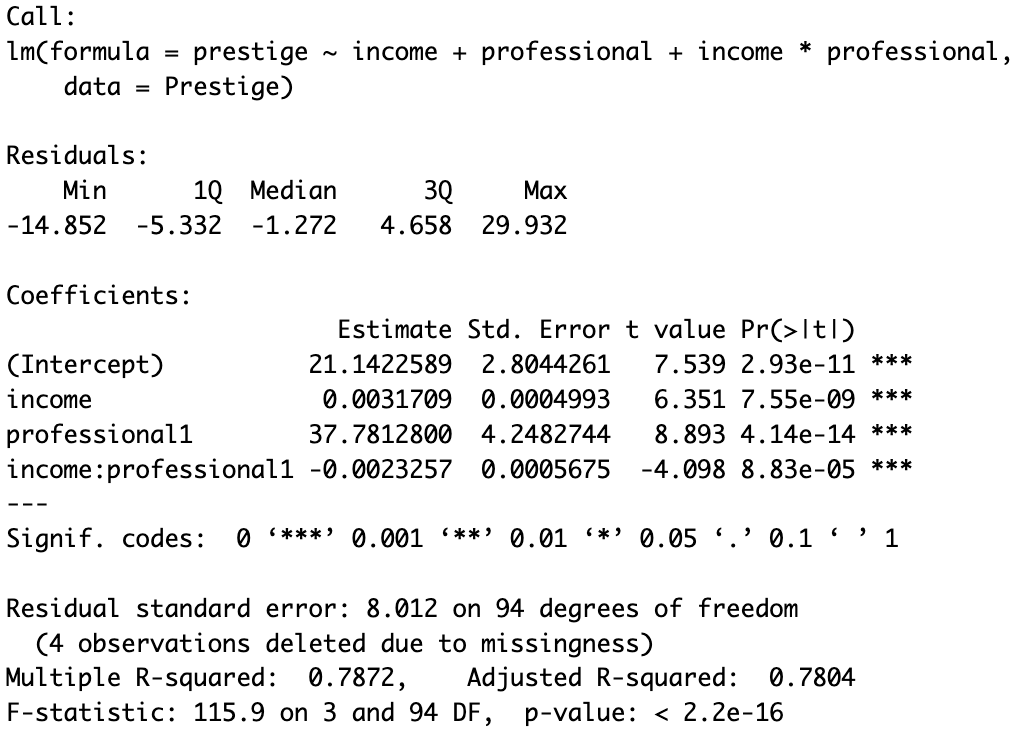
\includegraphics[width=1\textwidth]{Q1_Regression_Summary}
\end{figure}

	
	\vspace{6cm}
	\item [(c)]
	Write the prediction equation based on the result.
	
	$$E(y)= {\beta_0} + {\beta_1} \times \text{Income}+ {\beta_2} \times \text{Professional}+ {\beta_3}\times \text{(Income}\times \text{Professional)}$$
	
	$$E(y)= 21.142 + .003 \times \text{Income}+ 37.781 \times \text{Professional}- .002\times \text{(Income}\times \text{Professional)}$$
	
	\vspace{.25cm}
	\item [(d)]
	Interpret the coefficient for \texttt{income}.
	
	When someone does not have a professional career, a one unit increase in income (1 dollar), will on average result in a .003 increase in prestige
	
	\vspace{.25cm}	
	\item [(e)]
	Interpret the coefficient for \texttt{professional}.
	
	
	When income is 0, the change from not-professional (blue or white collar workers) to professional will, on average, result in a 37.781 increase in prestige. This is the difference in prestige between the groups (professional vs white/blue collar worker) when income is 0.
	
	\vspace{.25cm}	
	\item [(f)]
	What is the effect of a \$1,000 increase in income on prestige score for professional occupations? In other words, we are interested in the marginal effect of income when the variable \texttt{professional} takes the value of $1$. Calculate the change in $\hat{y}$ associated with a \$1,000 increase in income based on your answer for (c).
	
	$$E(y_1)= 21.142 + \text{(.003} \times \text{1000)}+ \text{(37.781} \times \text{1)}- \text{(.002}\times \text{1000}\times \text{1)} = 59.923$$
	
	$$E(y_0)= 21.142 + \text{(.003} \times \text{0)}+ \text{(37.781} \times \text{1)}- \text{(.002}\times \text{0}\times \text{1)} = 58.923$$
	
	$$E(y_1) - E(y_0) = 1$$
	
	There is a 1 unit increase in prestige when income increases from \$0 to \$1000 for individuals with professional careers. Professional individuals with an income of \$1,000 have a prestige of 59.923. Professional individuals with an income of \$0 have a prestige of 58.923.
	
			\lstinputlisting[language=R, firstline=68, lastline=74]{PS04_answers_CZ.R}
	\vspace{10cm}
	
	
	\item [(g)]
	What is the effect of changing one's occupations from non-professional to professional when her income is \$6,000? We are interested in the marginal effect of professional jobs when the variable \texttt{income} takes the value of $6,000$. Calculate the change in $\hat{y}$ based on your answer for (c).
	
	$$E(y_1)= 21.142 + \text{(.003} \times \text{6000)}+ \text{(37.781} \times \text{1)}- \text{(.002}\times \text{6000}\times \text{1)} = 64.923$$
	
	$$E(y_0)= 21.142 + \text{(.003} \times \text{6000)}+ \text{(37.781} \times \text{0)}- \text{(.002}\times \text{6000}\times \text{0)} = 39.142$$
	
	$$E(y_1) - E(y_0) = 25.781$$
	
	
	With an income of \$6,000, a change from non-professional to professional will increase prestige by 25.781, on average.
	
	\lstinputlisting[language=R, firstline=78, lastline=83]{PS04_answers_CZ.R}
\end{enumerate}

\newpage

\section*{Question 2: Political Science}
\vspace{.25cm}
\noindent 	Researchers are interested in learning the effect of all of those yard signs on voting preferences.\footnote{Donald P. Green, Jonathan	S. Krasno, Alexander Coppock, Benjamin D. Farrer,	Brandon Lenoir, Joshua N. Zingher. 2016. ``The effects of lawn signs on vote outcomes: Results from four randomized field experiments.'' Electoral Studies 41: 143-150. } Working with a campaign in Fairfax County, Virginia, 131 precincts were randomly divided into a treatment and control group. In 30 precincts, signs were posted around the precinct that read, ``For Sale: Terry McAuliffe. Don't Sellout Virgina on November 5.'' \\

Below is the result of a regression with two variables and a constant.  The dependent variable is the proportion of the vote that went to McAuliff's opponent Ken Cuccinelli. The first variable indicates whether a precinct was randomly assigned to have the sign against McAuliffe posted. The second variable indicates
a precinct that was adjacent to a precinct in the treatment group (since people in those precincts might be exposed to the signs).  \\

\vspace{.5cm}
\begin{table}[!htbp]
	\centering 
	\textbf{Impact of lawn signs on vote share}\\
	\begin{tabular}{@{\extracolsep{5pt}}lccc} 
		\\[-1.8ex] 
		\hline \\[-1.8ex]
		Precinct assigned lawn signs  (n=30)  & 0.042\\
		& (0.016) \\
		Precinct adjacent to lawn signs (n=76) & 0.042 \\
		&  (0.013) \\
		Constant  & 0.302\\
		& (0.011)
		\\
		\hline \\
	\end{tabular}\\
	\footnotesize{\textit{Notes:} $R^2$=0.094, N=131}
\end{table}

\vspace{.5cm}
\begin{enumerate}
	\item [(a)] Use the results from a linear regression to determine whether having these yard signs in a precinct affects vote share (e.g., conduct a hypothesis test with $\alpha = .05$).
	
	Assumptions for multiple regression:
	
	1. Samples from the population are independant and random samples
	
	2. Population distribution of the response variable for each group is normal
	
	3. Standard deviation of the population distribution is constant
	
	\newpage		
	
	Null hypothesis: $H_0$: The yard signs have no affect on vote share ($\beta_1 = 0$) \\
	Alternative hypothesis: $H_\alpha$: The yard signs have an affect on vote share ($\beta_1 \neq 0$)
	
	\vspace{.5cm}
	
	Test statistic = Estimate/SE = .042/.016 = 2.625
	
	P-value = 0.00972002
		\lstinputlisting[language=R, firstline=97, lastline=104]{PS04_answers_CZ.R}
	
	
	
	Conclusion: Based on the p-value of 0.00972002 and a .05 significance level, there is sufficient evidence to reject the null hypothesis that the yard signs have no affect on vote share. Therefore, a one unit increase in yard signs will, on average, increase vote share by .042.
	
		\vspace{1cm}			
	\item [(b)]  Use the results to determine whether being
	next to precincts with these yard signs affects vote
	share (e.g., conduct a hypothesis test with $\alpha = .05$).
	
	Assumptions for multiple regression:
	
	1. Samples from the population are independant and random samples
	
	2. Population distribution of the response variable for each group is normal
	
	3. Standard deviation of the population distribution is constant
	
			\vspace{.25cm}			
		Null hypothesis: $H_0$: The yard signs in adjacent precincts have no affect on vote share ($\beta_2 = 0$) \\
	Alternative hypothesis: $H_\alpha$: The yard signs in adjacent precincts have an affect on vote share ($\beta_2 \neq 0$)
	
				\vspace{.25cm}			
	Test statistic = Estimate/SE = .042/.013 = 3.230769
	
	P-value = 0.00156946
	
		\lstinputlisting[language=R, firstline=110, lastline=113]{PS04_answers_CZ.R}
	
	\newpage
	
	Conclusion: Based on the p-value of 0.00156946 and a .05 significance level, there is sufficient evidence to reject the null hypothesis that the adjacent precincts with yard signs have no affect on vote share. Therefore, a one unit increase in yard signs in adjacent precincts will, on average, increase vote share by .042.
	
	
	\vspace{1cm}
	\item [(c)] Interpret the coefficient for the constant term substantively.
	\vspace{.5cm}
	
	The baseline group, a district with no assigned lawn signs and not adjacent to a lawn sign precinct, is expected to have a vote share of .302 per Cuccinelli. The t-stat for the constant is 27.45, which is large and significant when compared to the test statistics calculated for the precinct assigned lawn signs and precinct adjacent to lawn signs coefficients. 
			\lstinputlisting[language=R, firstline=121, lastline=121]{PS04_answers_CZ.R}
	
	\vspace{1cm}
	\item [(d)] Evaluate the model fit for this regression.  What does this	tell us about the importance of yard signs versus other factors that are not modeled?
	
	The $R^2$ for this regression is .094. Given that $R^2$ will always fall between 0 and 1, this is a very small $R^2$. Only 9.4\% the variation in vote share is explained by the yard signs in or adjacent to precincts. There are other factors that need to be accounted for when trying to explain vote share besides just yard sign placement. 
\end{enumerate}  


\end{document}
